\documentclass{beamer}
\usepackage{tikz}

% internal parameters
\usetheme{Copenhagen}
\usecolortheme{default}
\setbeamertemplate{caption}[numbered]

% packages
\usepackage{graphics}
\usepackage{amsmath}
\usepackage{xcolor}
\usepackage{physics}
\usepackage{fontawesome}
\usepackage{mathrsfs}  
\usepackage{multirow}


\title[Wobbling Motion]{New Results Concerning Collective Motion in Triaxial Nuclei}
\author[Robert POENARU]{Robert POENARU\inst{1,2}}

\institute[VFU]
{
  \inst{1}%
  Dept. of Th. Phys. @ IFIN-HH\\
  Magurele, Romania
  \and
  \inst{2}%
  Doctoral School of Physics\\
  Bucharest, Romania
}

\date{\textit{UB Faculty of Physics Meeting}\\\textit{\today}}

%------------------------------------------------------------
%The next block of commands puts the table of contents at the 
%beginning of each section and highlights the current section:
% \AtBeginSection[]
% {
%   \begin{frame}
%     \frametitle{Table of Contents}
%     \tableofcontents[currentsection]
%   \end{frame}
% }

%------------------------------------------------------------
\begin{document}
%---------------------------------------------------------
\frame{\titlepage}
\begin{frame}
  \frametitle{Table of Contents}
  \tableofcontents
\end{frame}

\section{Nuclear Shapes}
\begin{frame}{Nuclear Deformation}
\par Most of the nuclei are either \emph{spherical} or \emph{axially symmetric} in their ground-state.
\par Deformation parameter $\beta$ (\textit{Bohr, 1969}): preserves axial symmetry
\begin{figure}
  \centering
  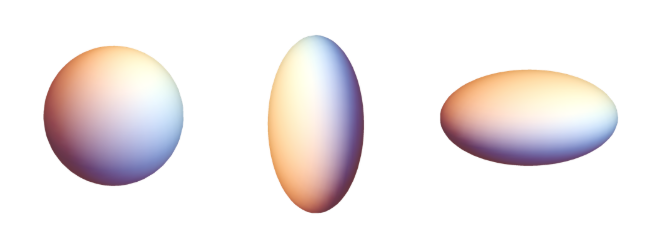
\includegraphics[width=0.99\textwidth]{Figs/nuclear_shapes.png}
  \caption{\textbf{spherical:} $\beta=0$\ \textbf{prolate:} $\beta>0$\ \textbf{oblate:} $\beta<0$}
\end{figure}
\end{frame}

\begin{frame}
  \frametitle{Nuclear Triaxiality}
  \begin{alertblock}{Non-axial shape}
    \par Deviations from symmetric shapes can occur across the chart of nuclides $\to$ \textbf{triaxial nuclei}.
    \par The triaxiality parameter $\gamma$ (\textit{Bohr, 1969}): departure from axial symmetry
  \end{alertblock}
  \begin{figure}
    \centering
    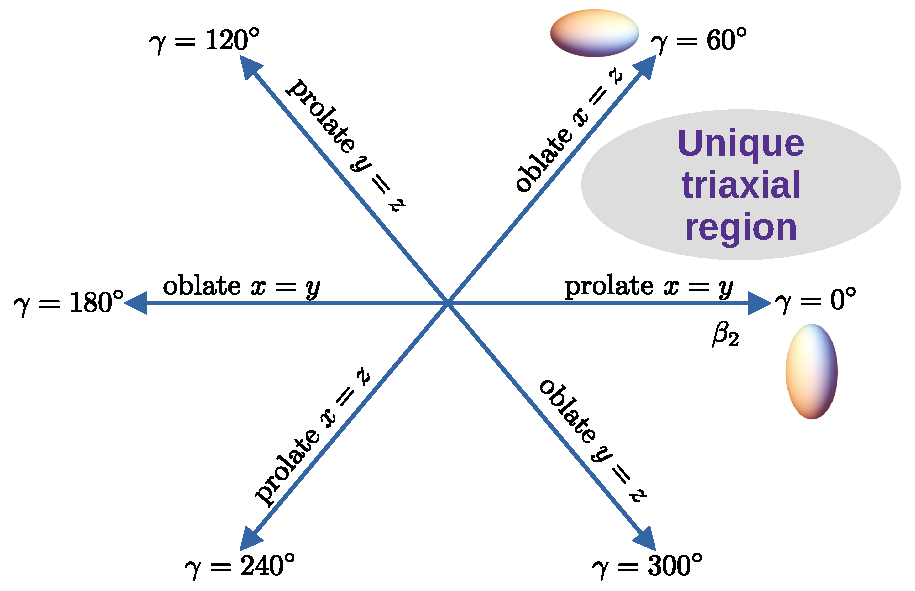
\includegraphics[scale=0.42]{Figs/nice_diagram.pdf}
    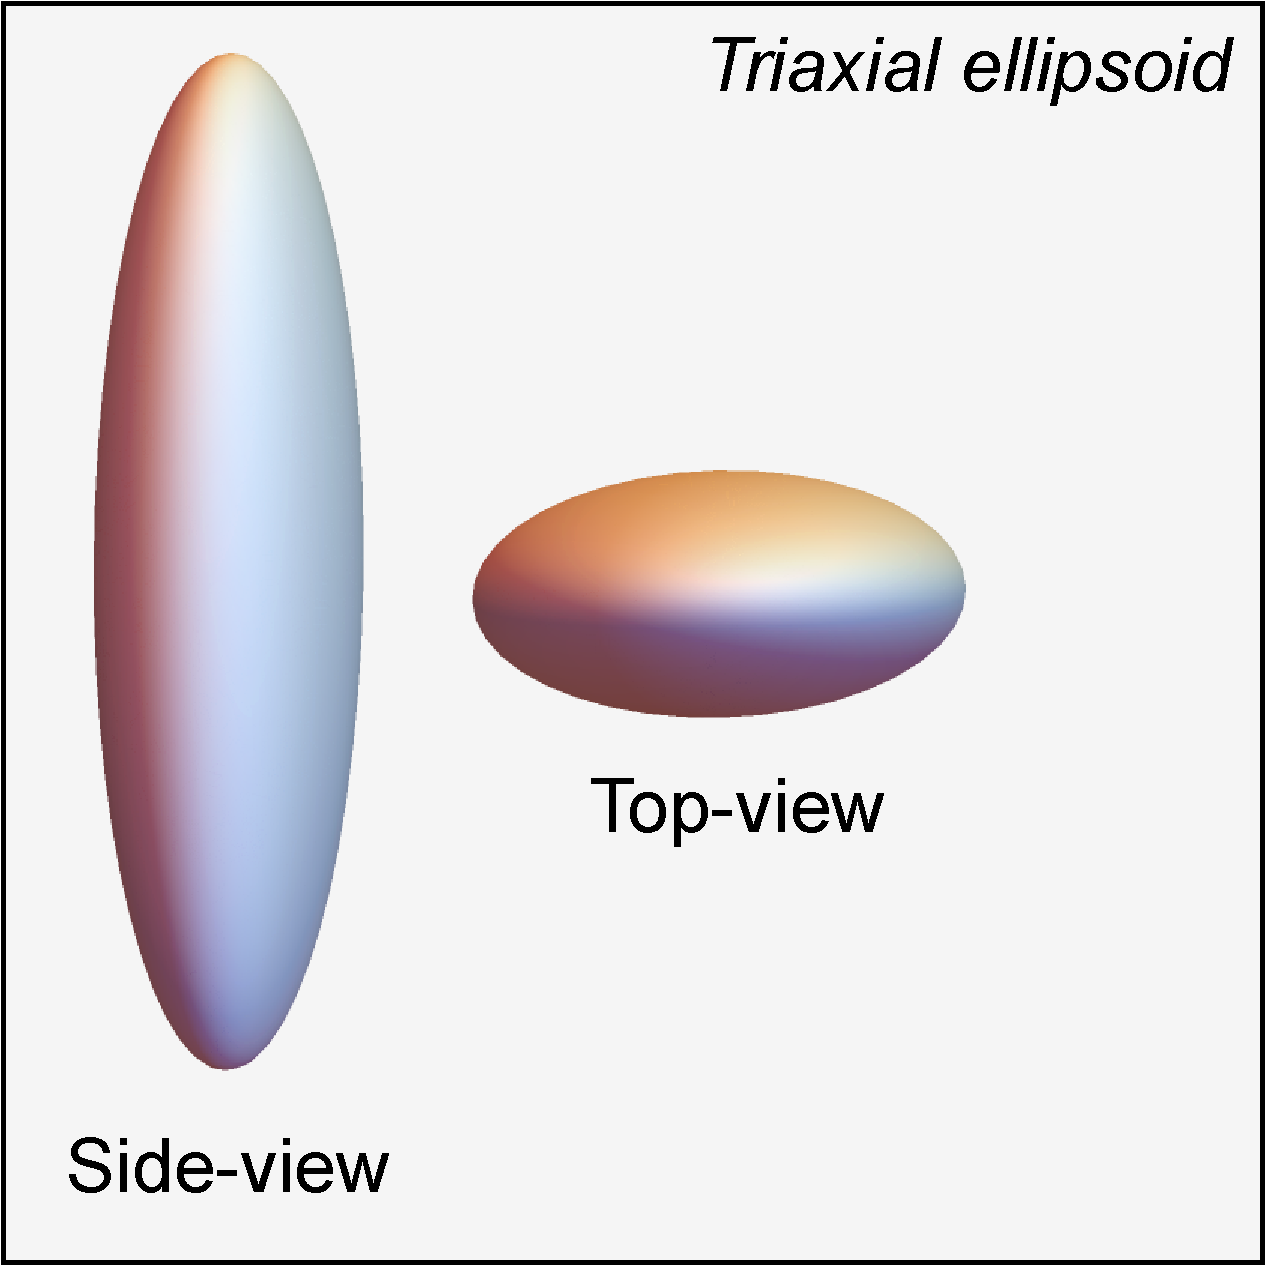
\includegraphics[scale=0.19]{Figs/triaxial-shape.pdf}
    % \caption{The $(\beta,\gamma)$ plane divided into six equivalent parts, depicting nuclear surfaces.}
  \end{figure}
\end{frame}

\begin{frame}
  \frametitle{Fingerprints for Triaxiality}
  \begin{itemize}
    \item Experimentally, stable triaxial nuclei represent a real challenge
    \item Clear signatures for confirming stable triaxiality in nuclei
    \begin{enumerate}
      \item Chiral symmetry breaking (\textit{Frauendorf, 1997})
      \item \textbf{Wobbling motion} (\textit{Bohr \& Mottelson, 1975})
    \end{enumerate}
  \end{itemize}
  \begin{block}{Wobbling Motion (WM)}
    \begin{itemize}
      \item Unique to non-axial nuclei
      \item Predicted 50 years ago for even-$A$ nuclei
      \item First experimental evidence for $^{163}$Lu (\textit{Ødegård}, 2001)
      \item Currently: confirmed wobblers within the mass regions $A\approx[100,130,160,180]$.
    \end{itemize}
  \end{block}
\end{frame}

\begin{frame}
  \frametitle{Energy of Deformed Nuclei}
    \begin{block}{Collective Motion}
      \begin{itemize}
        \item A nucleus - \emph{droplet} - can generate angular momentum from the rotation and vibration of the droplet itself
        \item Each individual nucleon contributes to the total angular momentum $\rightarrow$ \emph{collectiveness}
        \item \faWarning Rotation can occur only if the nuclear potential is \emph{deformed}
      \end{itemize}
    \end{block}
    \begin{figure}
      \centering
      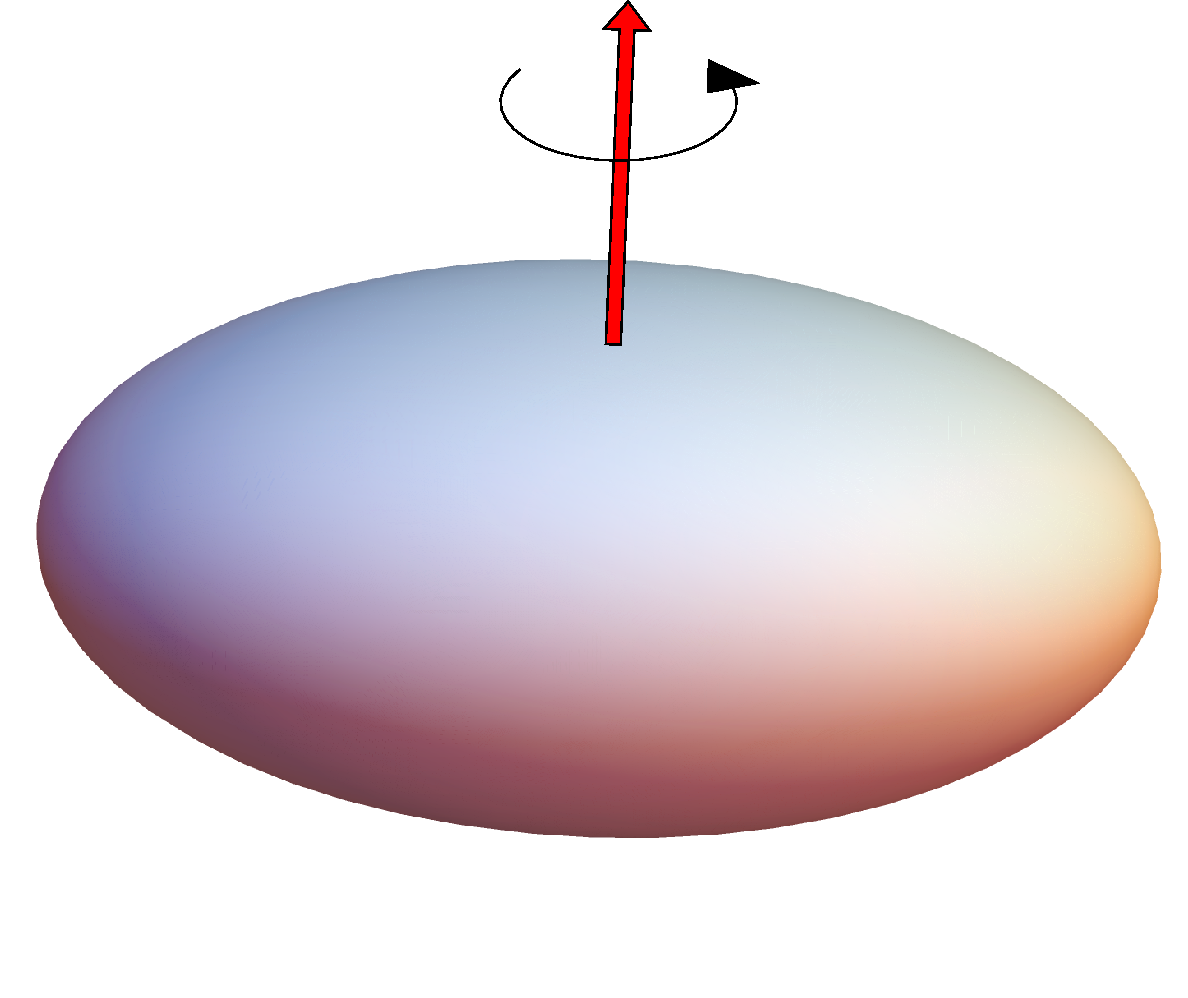
\includegraphics[scale=0.22]{Figs/collective-rotation.pdf}
    \end{figure}
\end{frame}

\begin{frame}
  \frametitle{Triaxial Rotor Energy}
  \begin{itemize}
    \item A triaxial nucleus can rotate about any of the three axes
    \item Rotation about the axis with \textbf{the largest moment of inertia} (MOI) is energetically the most favorable: $E_\text{rot}\propto\frac{\hbar^2}{2\mathcal{I}_\text{max}}I(I+1 )$
    \item MOI anisotropy $\rightarrow$ the \emph{main rotation} around $\mathcal{J}_\text{max}$ is disturbed by the other two axes $\rightarrow$ {\color{red}\emph{total motion of the rotating nucleus has an oscillating behavior}}
  \end{itemize}
  \begin{figure}
    \centering
    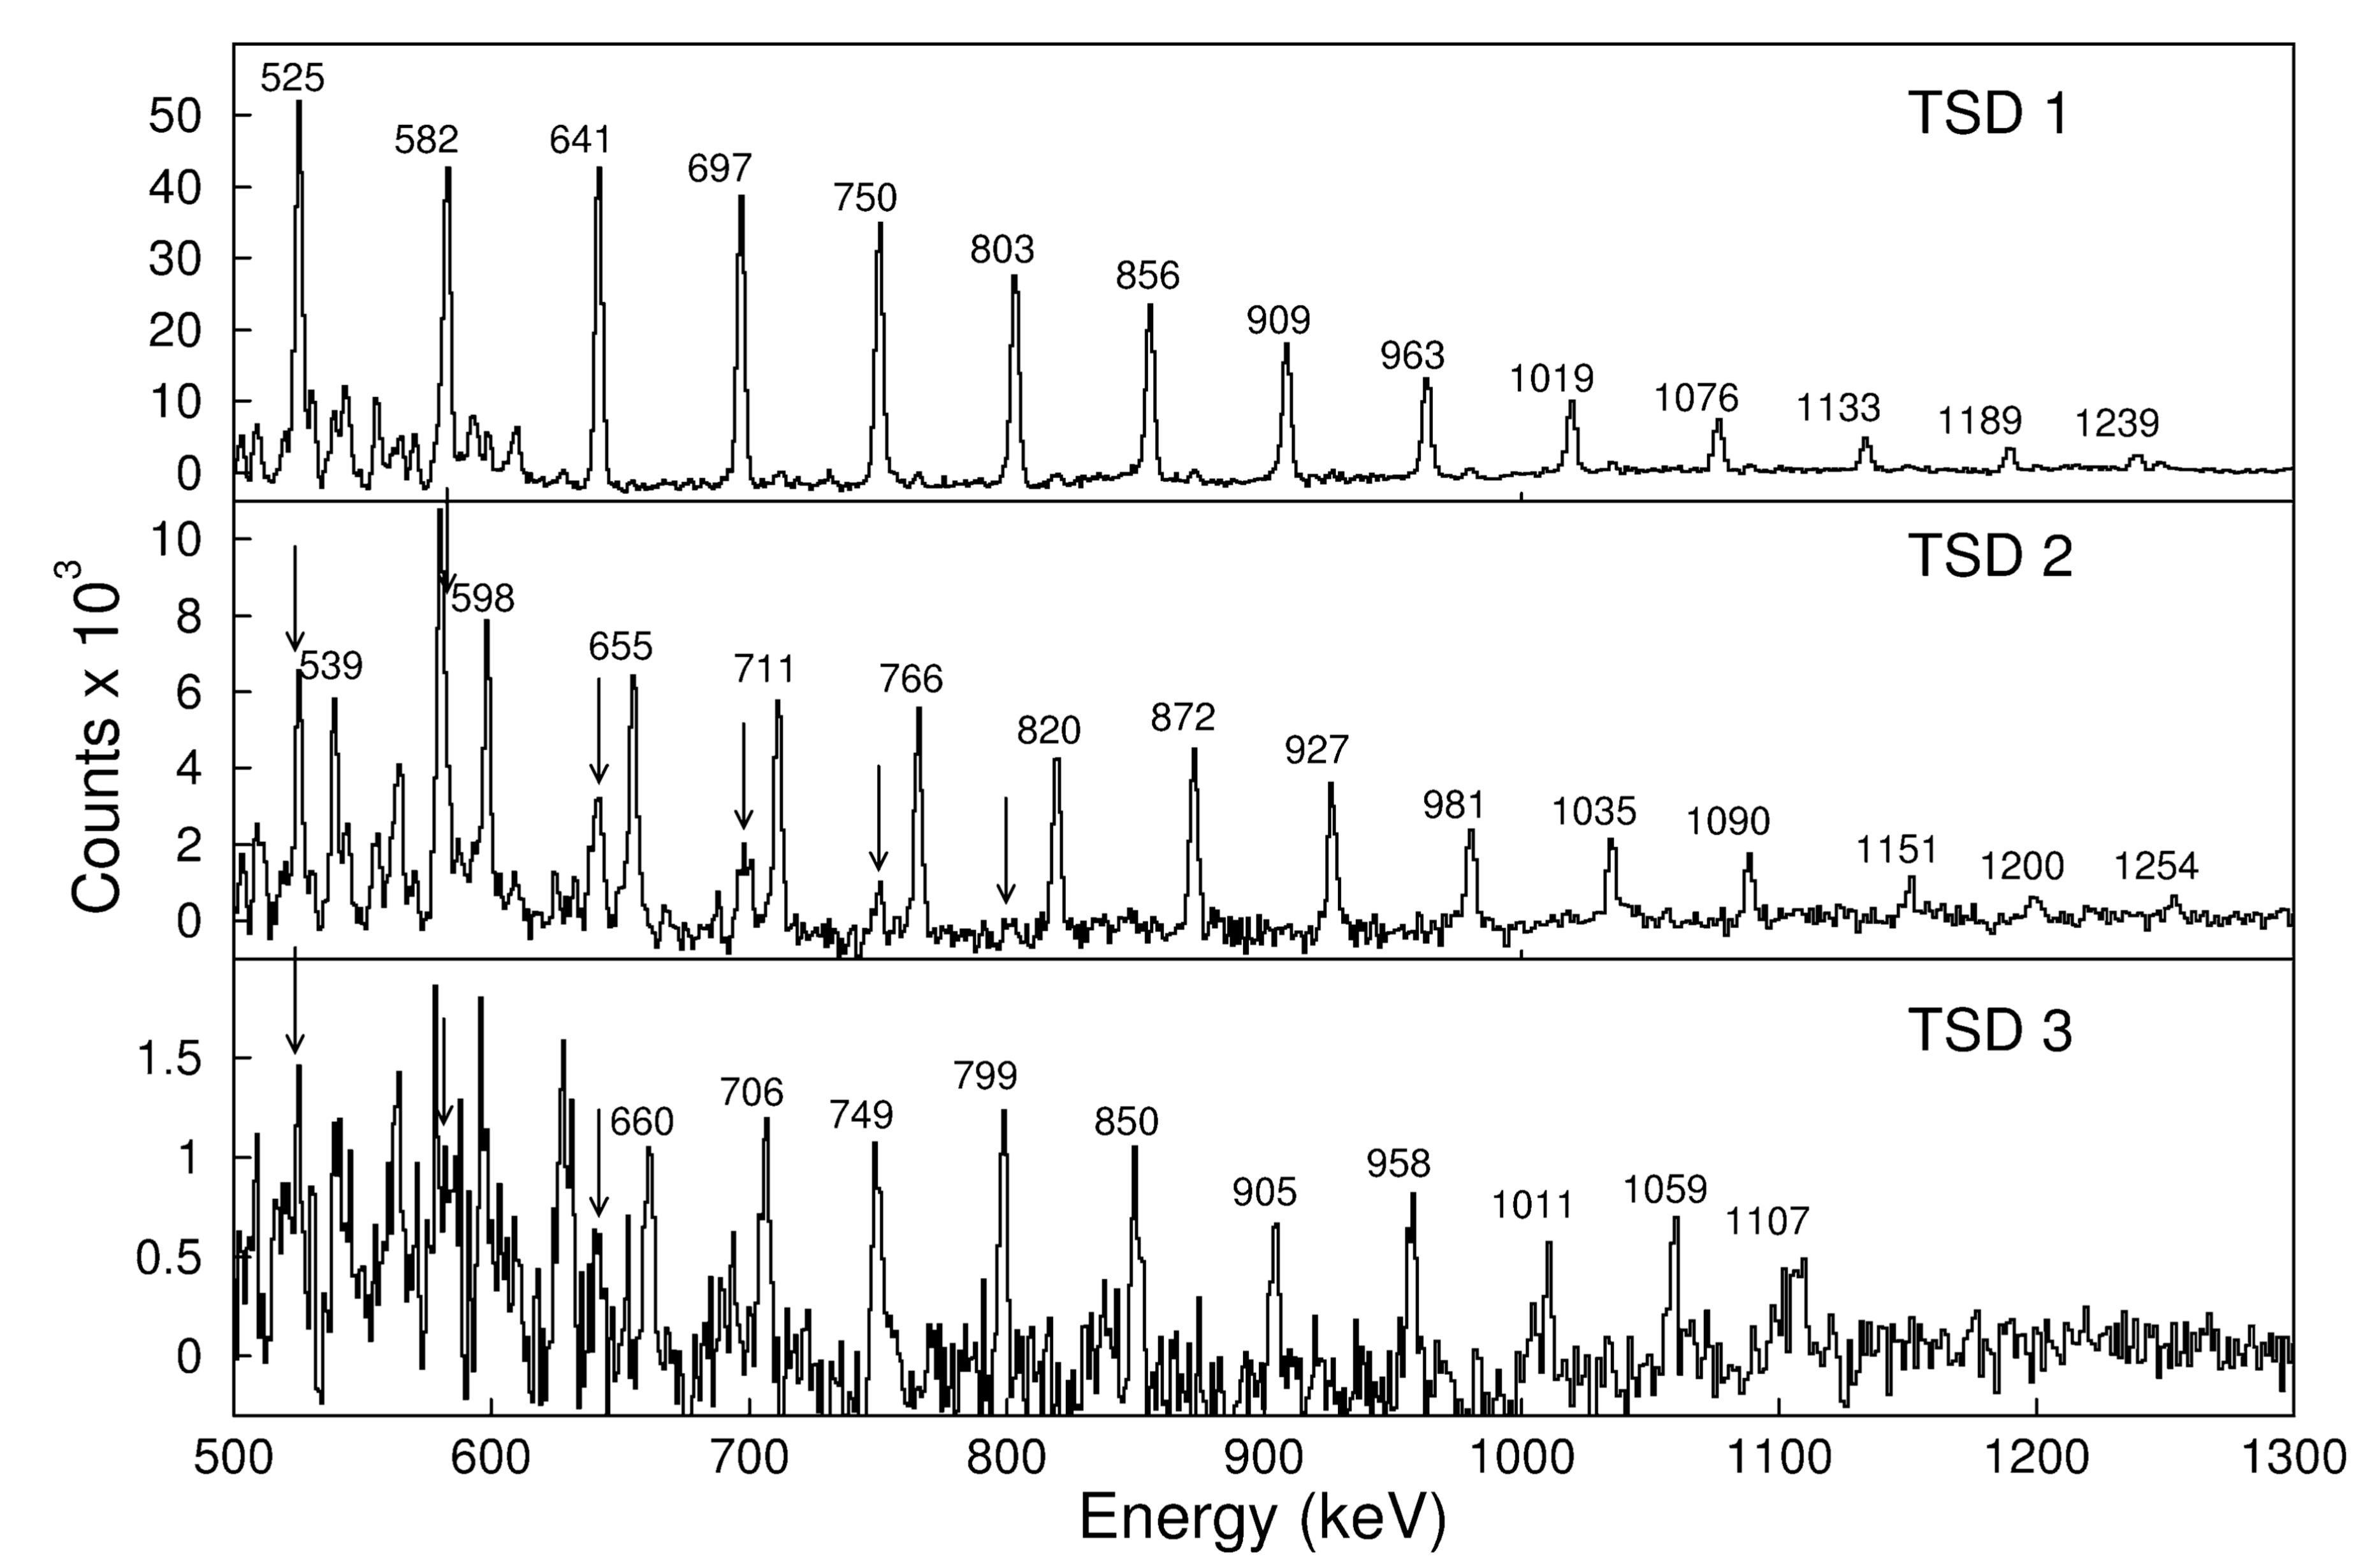
\includegraphics[scale=0.09]{Figs/collective-spectra.pdf}
    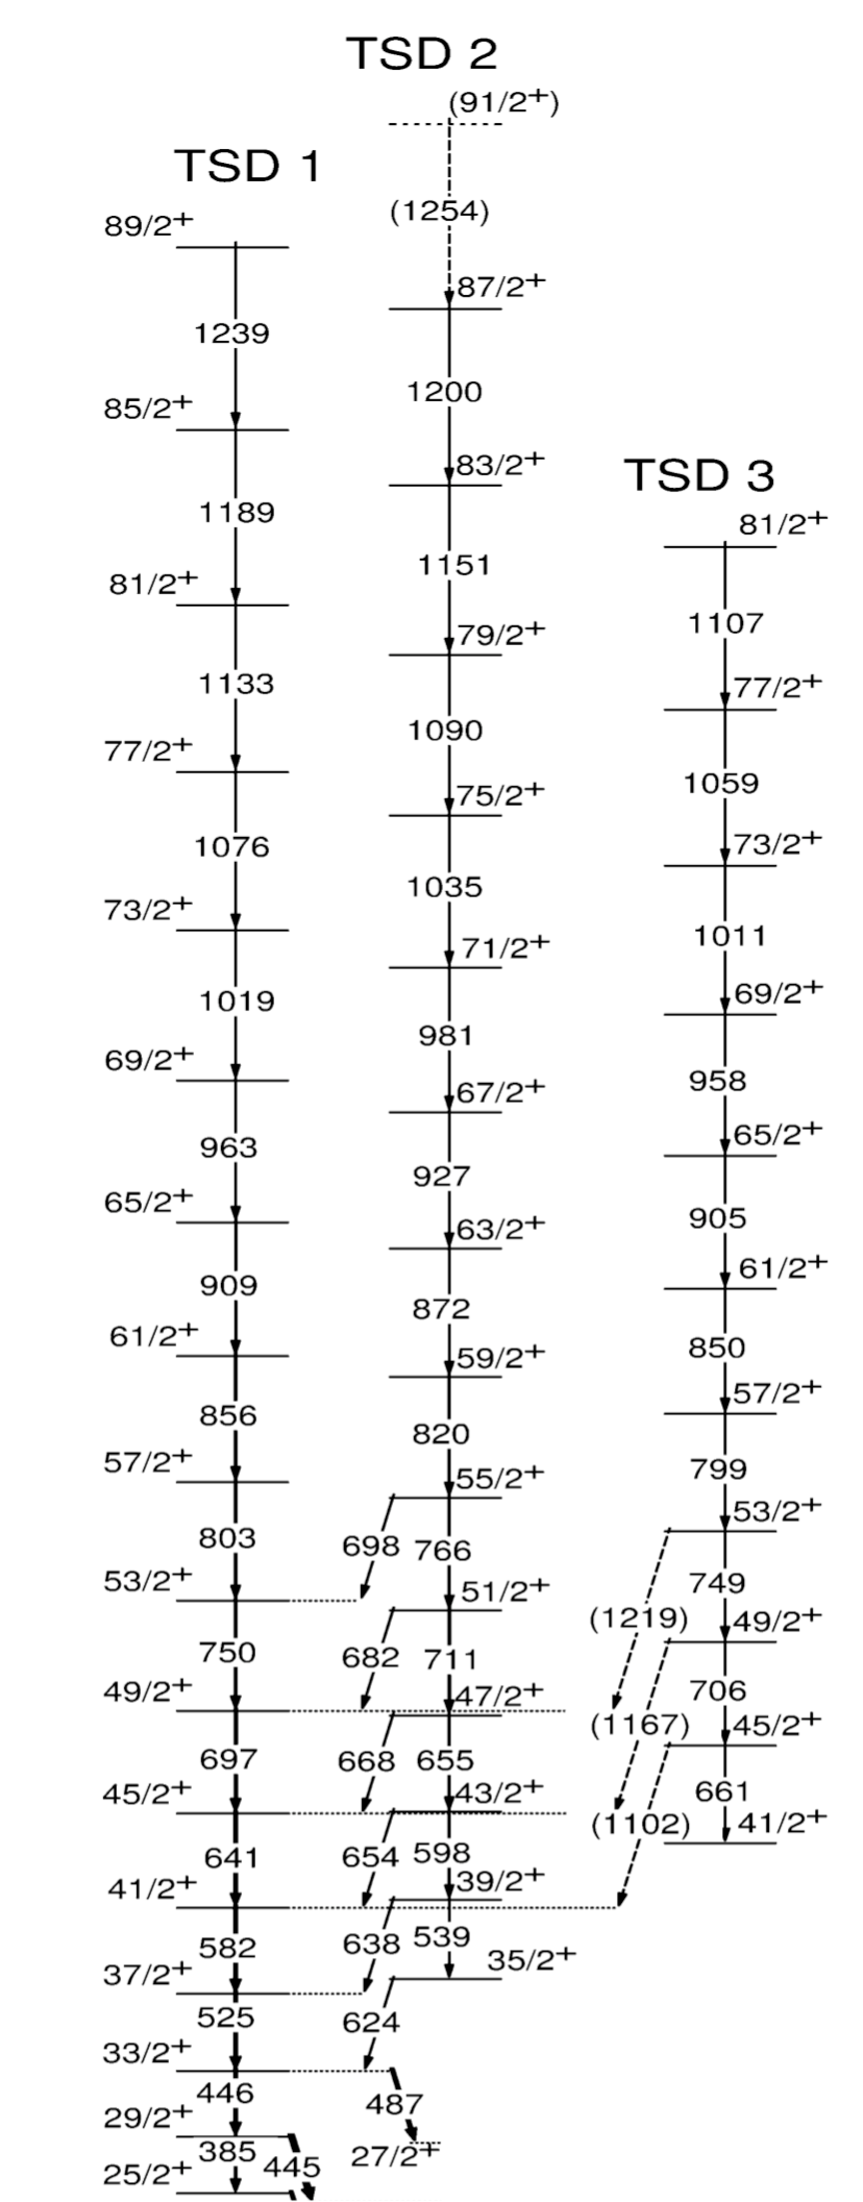
\includegraphics[scale=0.1]{Figs/collective-levels.pdf}
  \end{figure}
  \tiny{\textit{Figures from Ødegård et al., 2001}}
\end{frame}

\begin{frame}
  \frametitle{Wobbling Motion}
\begin{itemize}
  \item Total angular momentum $\mathbf{I}$ disaligned w.r.t. body-fixed axes
  \item The a.m. \textbf{precesses} and \textbf{wobbles} around the axis with $\mathcal{J}_\text{max}$
  \item The precession of $\mathbf{I}$ can increase by \textbf{tilting} 
  \item Tilting by an energy quanta $\sim$ \emph{vibrational character} $\rightarrow$ \textbf{wobbling phonon} $n_w=0,1,2...$
\end{itemize}
  \begin{figure}
    \centering
    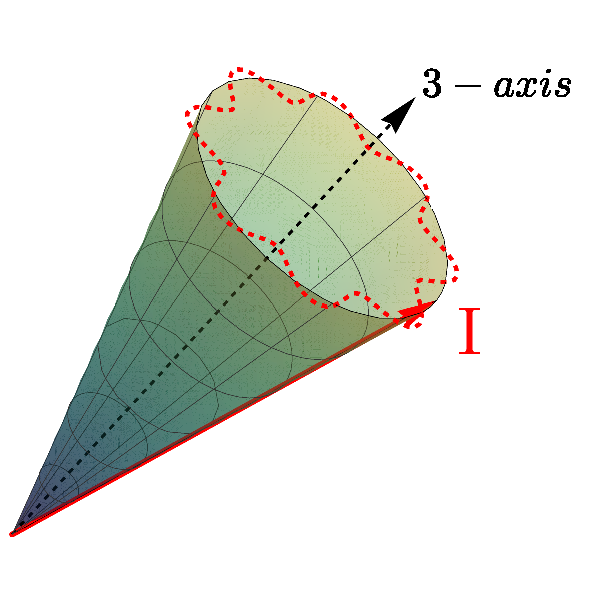
\includegraphics[scale=0.4]{Figs/precessional_cone_2.pdf}
    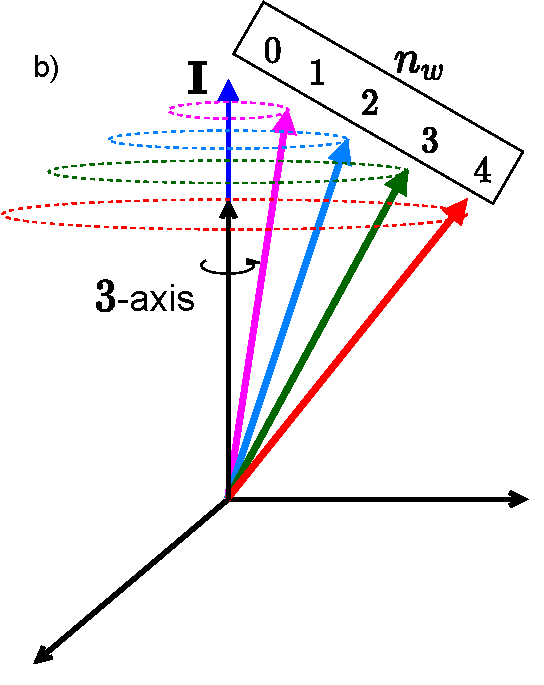
\includegraphics[scale=0.35]{Figs/wobbling_n_schematic-2.pdf}
  \end{figure}
\end{frame}

\begin{frame}
  \frametitle{Wobbling Spectrum}
\begin{block}{Even-$A$ Nuclei}
  \begin{itemize}
    \item Employing the Harmonic Approximation \textit{(Bohr, 1969)}
    \item $\hat{H}$ composed of a {\color{red}\emph{rotational}} part and {\color{blue}\emph{harmonic oscillation}} (i.e., wobbling) part:
  \end{itemize}
  \begin{align}
    \hat{H}={\color{red}\frac{\hbar^2}{2\mathcal{J}_\text{max}}I(I+1)}+{\color{blue}\hbar\omega_\text{wob}\left(n_w+\frac{1}{2}\right)}\ , n=0,1,2,\dots
    \label{wobbling-hamiltonian-even-A}
  \end{align}
\end{block}
\begin{figure}
  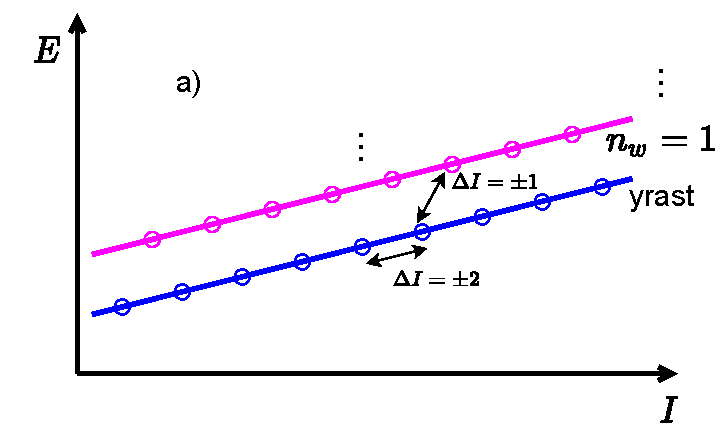
\includegraphics[scale=0.4]{Figs/wobbling_n_schematic-1.pdf}
  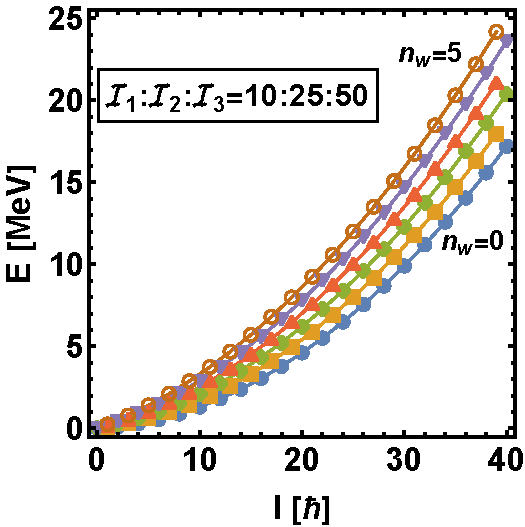
\includegraphics[scale=0.35]{Figs/wobblingFreq-evenA.pdf}
\end{figure}
\end{frame}

\begin{frame}
  \frametitle{New Results for A=130}
  \begin{minipage}{.8\textwidth}
    \begin{block}{Recent findings for even-even nuclei}
      \begin{itemize}
        \item Two wobbling bands have been identified experimentally in \textbf{$^\mathbf{130}$Ba} (\textit{Petrache et al., 2019})
        \item DFT+PRM description of the wobbling motion described the excited spectra (\textit{Chen et al., 2019})
        \item Stable triaxiality for $\beta=0.24$ and $\gamma=21.5^\circ$
        \item Infer spin-dependence for $\mathcal{J}_{1,2,3}$
      \end{itemize}
    \end{block}
  \end{minipage}%
  \begin{minipage}{.2\textwidth}
    \begin{figure}
      \centering
      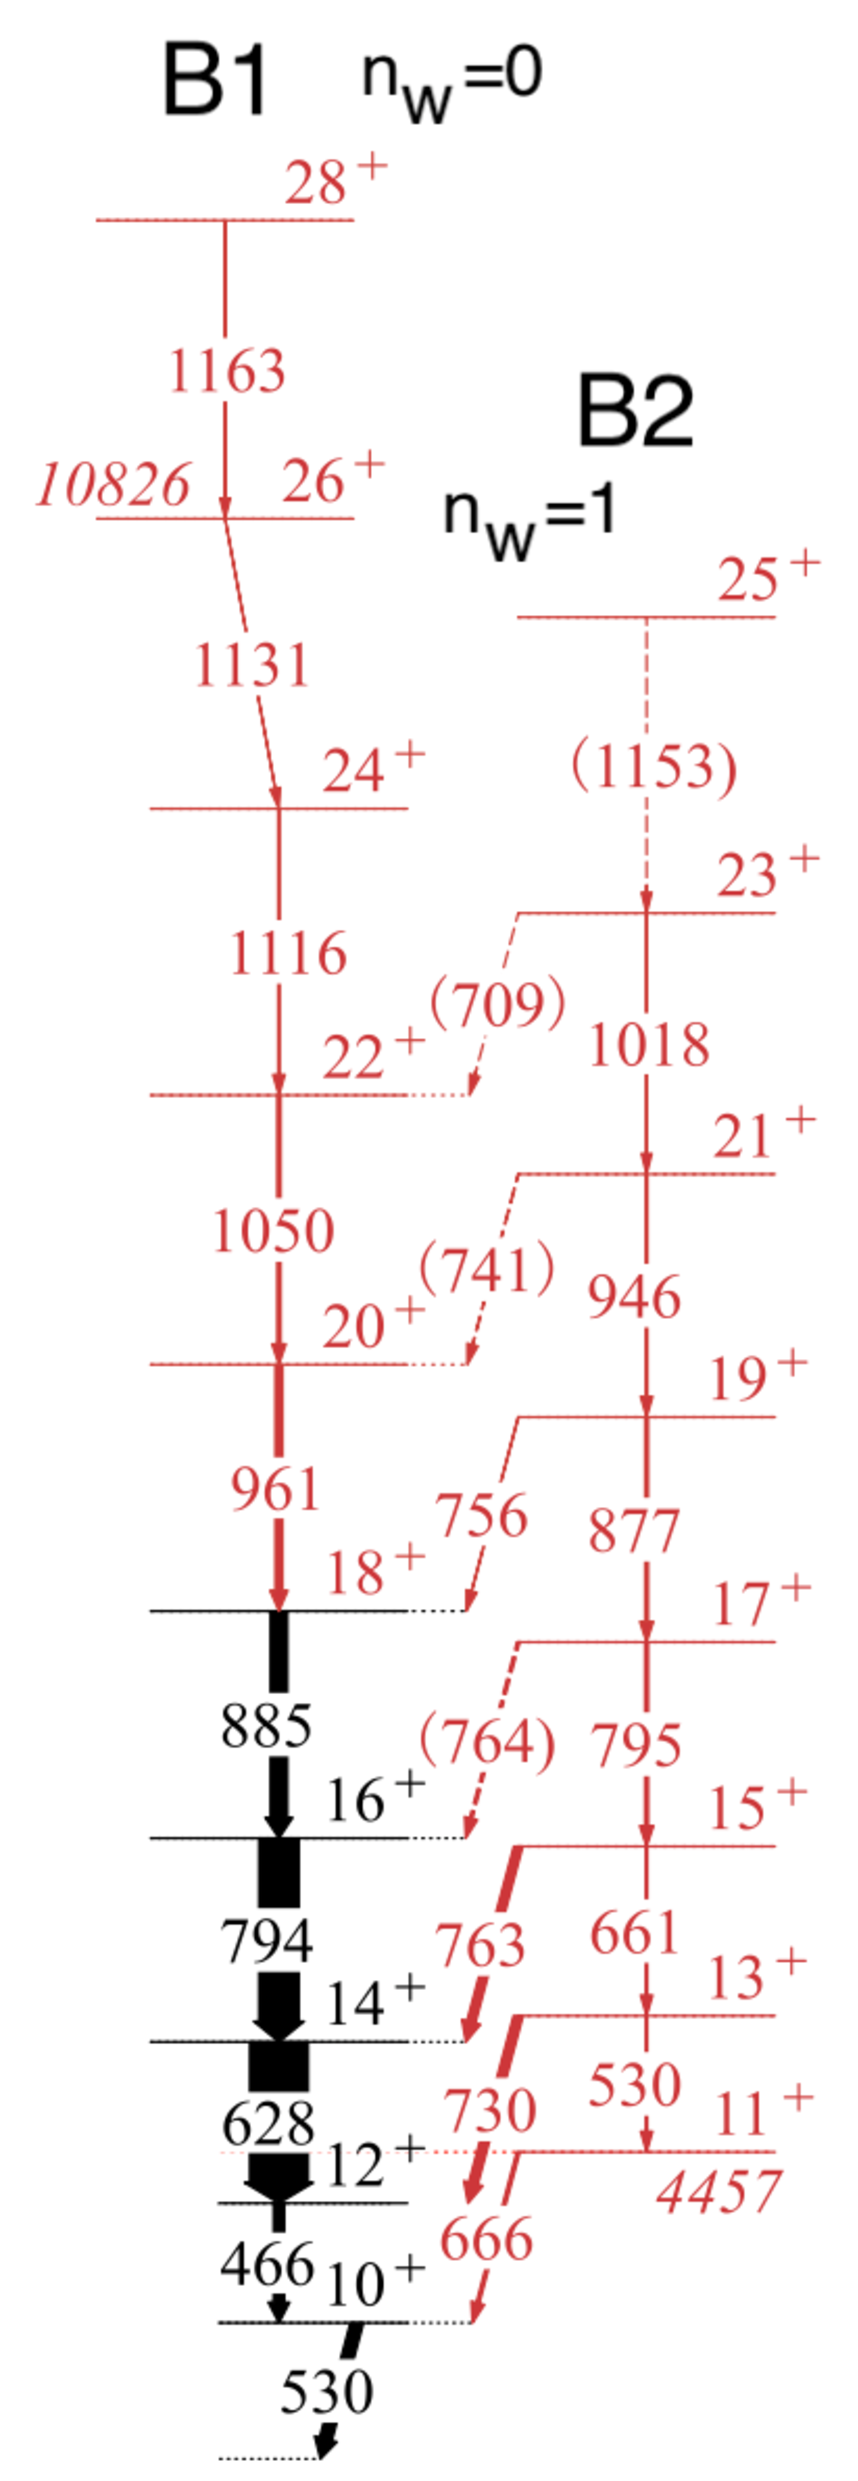
\includegraphics[scale=0.13]{Figs/ba-130-level-scheme.pdf}
      \tiny{\textit{Figure from Petrache et al., 2019}}
    \end{figure}
  \end{minipage}
\end{frame}

\begin{frame}
  \frametitle{New Results for A=130 II}
  \begin{columns}
    \begin{column}{0.8\textwidth}
      \begin{alertblock}{Harmonic Approximation}
        \begin{itemize}
          \item Employed an energy spectrum of harmonic type according to Eq. \ref{wobbling-hamiltonian-even-A}:
          \begin{align}
            E_{I,n_w}={\color{red}\frac{\hbar^2}{2\mathcal{J}_3}I(I+1)}+{\color{blue}\hbar\omega_\text{wob}(n_w+\frac{1}{2})}
          \end{align}
          \item wobbling frequency - linear dependence on $I$ (fixed MOI ordering $\mathcal{J}_3>\mathcal{J}_{1,2}$)
          \begin{align}
            {\color{blue}\hbar\omega_\text{wob}(I)=2f(\mathcal{J}_1,\mathcal{J}_2,\mathcal{J}_3)\cdot I}
          \end{align}
        \end{itemize}
      \end{alertblock}
  \end{column}
  \begin{column}{0.2\textwidth}
    \begin{figure}
      \centering
      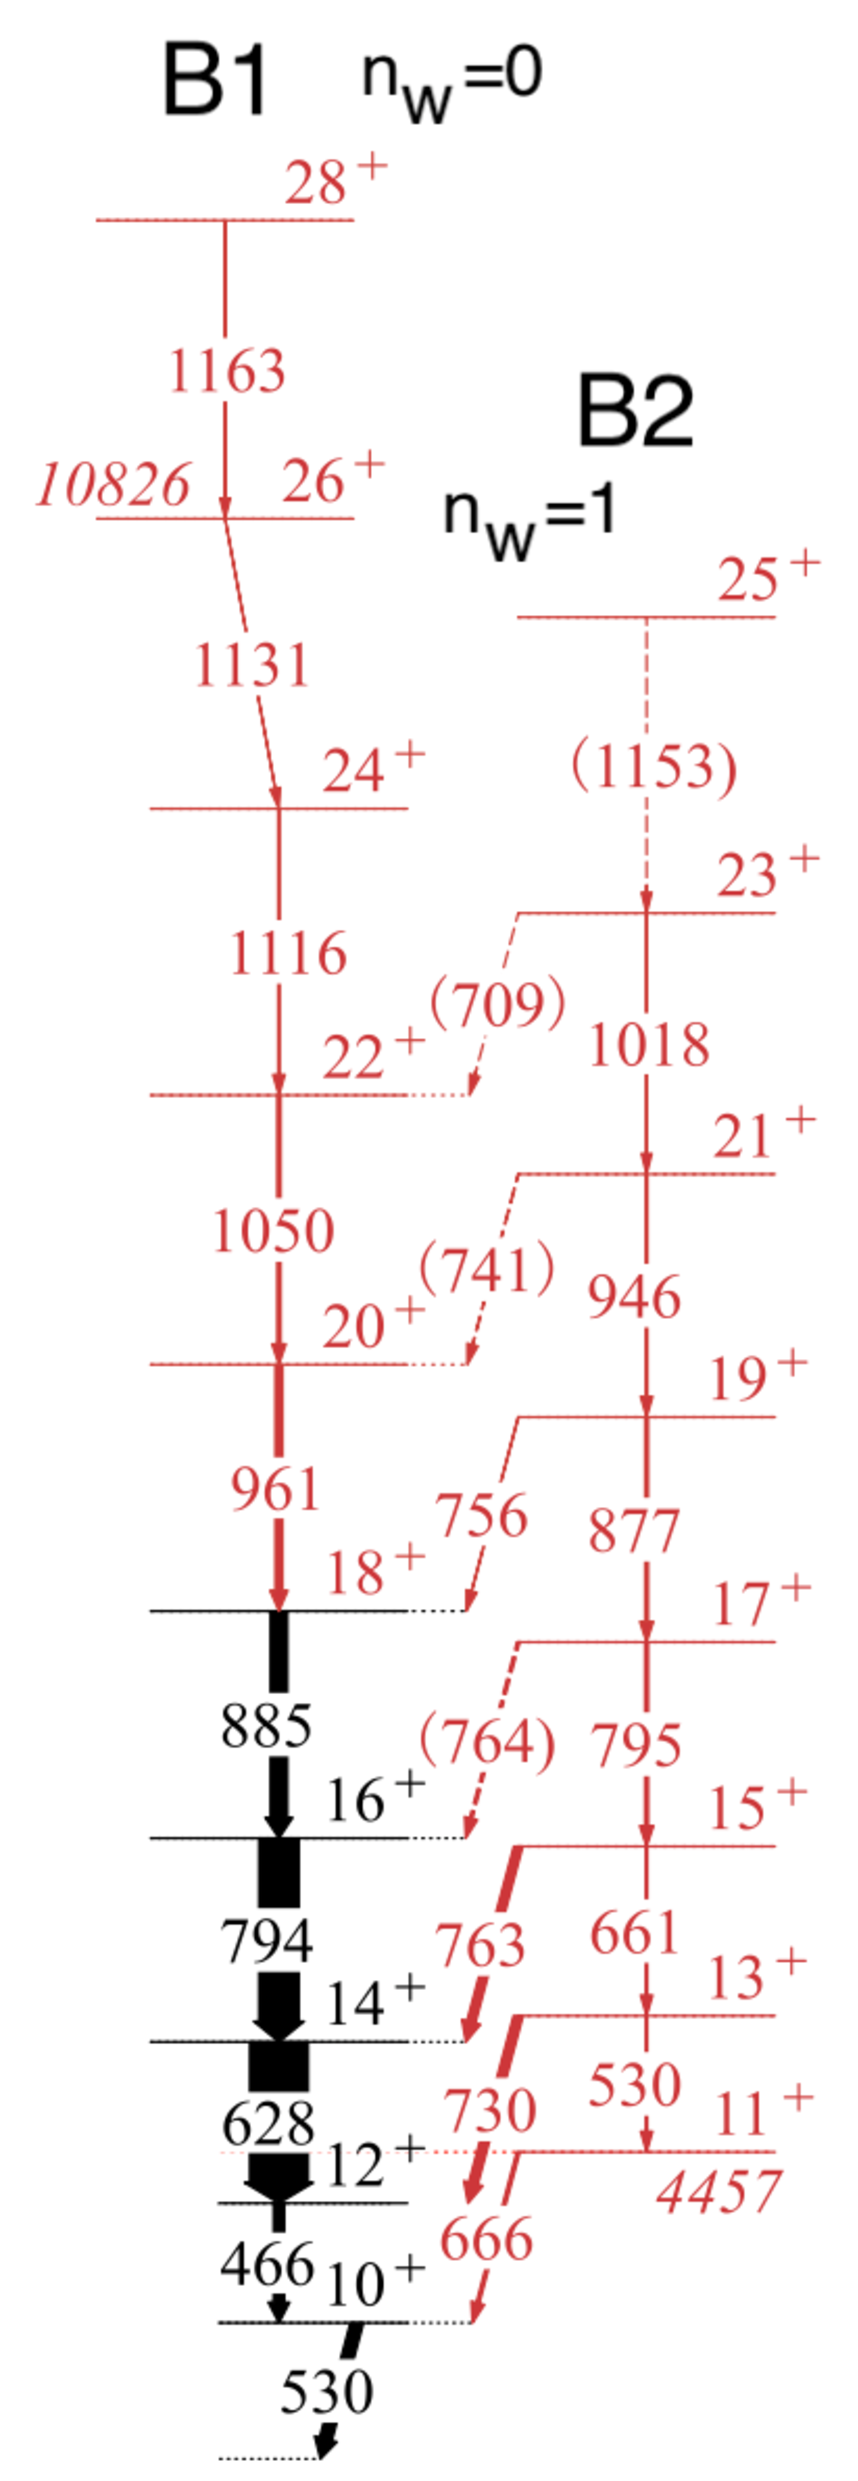
\includegraphics[scale=0.13]{Figs/ba-130-level-scheme.pdf}
      \tiny{\textit{Figure from Petrache et al., 2019}}
    \end{figure}
  \end{column}
  \end{columns}
\end{frame}

\begin{frame}
  \frametitle{New Results for A=130 III}
  \begin{columns}
    \begin{column}{0.75\textwidth}
      \begin{alertblock}{Harmonic Approximation}
        \begin{itemize}
          \item Reproduced the excited spectra for $\{B1,B2\}$
          \item Fix a \emph{free parameter set}: $\mathcal{P}=\left[\mathcal{J}_1,\mathcal{J}_2,\mathcal{J}_3\right]$
          \item Adopt a fitting procedure:
          \begin{align}
            \chi^2=\frac{1}{N_T}\sum_{i=1}^{N_T}\frac{\left(E_\text{exp}^{(i)}-E_\text{th}^{(i)}\right)}{E_\text{exp}^{(i)}}
          \end{align}
          % \item $\texttt{min}\left[\chi^2\right]\longrightarrow\mathcal{P}_\text{fit}$.
        \end{itemize}
      \end{alertblock}
      \begin{exampleblock}{Results for $^{130}$Ba \textbf{PRELIMINARY!}}
        \begin{table}
          \centering
          \begin{tabular}{|c|c|c|c|}
          \hline
          $\mathcal{J}_1^\text{fit}$ & $\mathcal{J}_2^\text{fit}$ & $\mathcal{J}_3^\text{fit}$ & \multirow{2}{*}{$\left[\hbar^2\text{MeV}^{-1}\right]$} \\ \cline{1-3}
          27                         & 22                         & 43                         &                                                       \\ \hline
          \end{tabular}
          \end{table}
      \end{exampleblock}
  \end{column}
  \begin{column}{0.25\textwidth}
    \begin{figure}
      \centering
      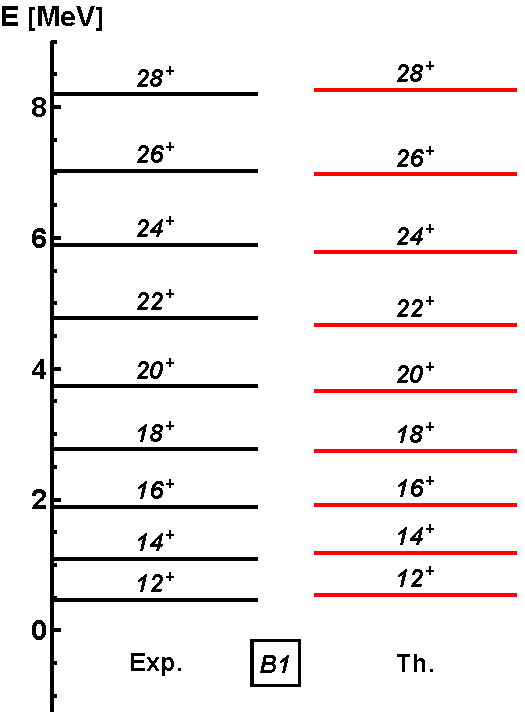
\includegraphics[scale=0.285]{Figs/ba130-band1.pdf}
      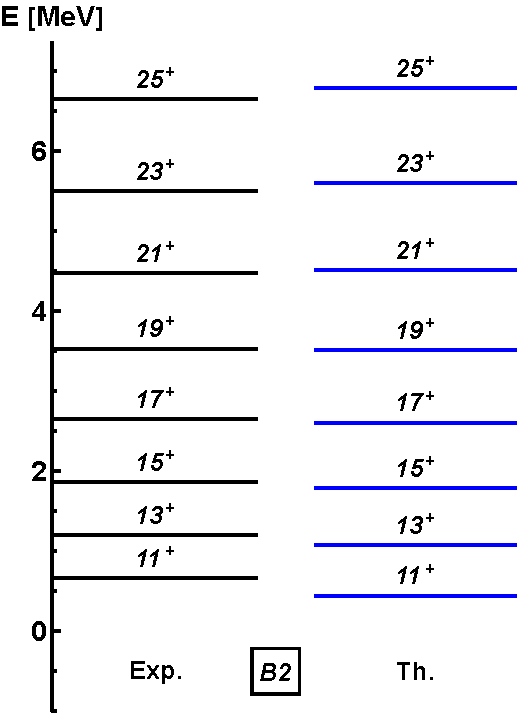
\includegraphics[scale=0.285]{Figs/ba130-band2.pdf}
      \tiny{\emph{Poenaru, 2022, unpublished}}
    \end{figure}
  \end{column}
\end{columns}
\end{frame}

\begin{frame}
  \frametitle{New Results for A=130 IV}
  \begin{itemize}
    \item \textbf{Left:} Wobbling energy* $E_\text{wob}(I)=E_\text{B2}(I)-E_\text{B1}(I)$
    \item \textbf{Center:} Rotational frequency $\hbar\omega_\text{rot}$ - collective
    \item \textbf{Right:} Interband transition probabilities $I_\text{B2}\to I_\text{B1}$
  \end{itemize}
  \begin{figure}
    \centering
    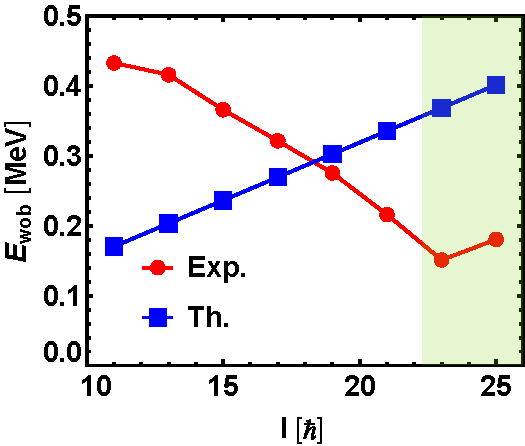
\includegraphics[scale=0.4]{Figs/ba130-wobbling-energies-edited.pdf}
    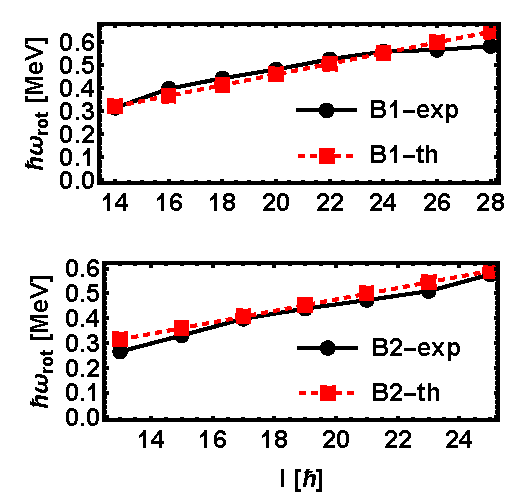
\includegraphics[scale=0.36]{Figs/ba130-rotational-frequencies.pdf}
    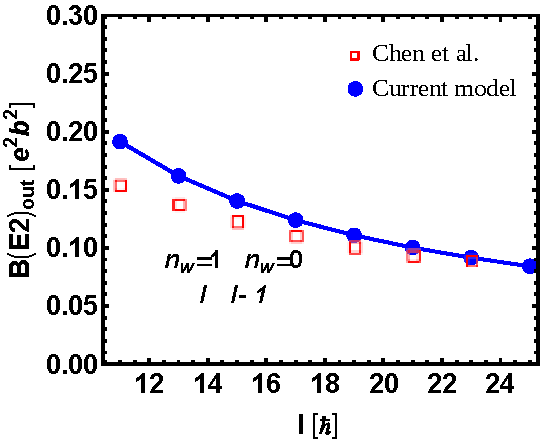
\includegraphics[scale=0.4]{Figs/ba130-EM.pdf}
    \tiny{\emph{Poenaru, 2022, unpublished}}
  \end{figure}
\end{frame}

\begin{frame}
  \frametitle{Electromagnetic transitions}
  \begin{columns}
    \begin{column}{0.75\textwidth}
  \begin{itemize}
    \item Deformation parameters $\beta=0.24$ and $\gamma=21.5^\circ$ were adopted for \emph{quadrupole moments} and \emph{transition probabilities}
    \item \par PRM values are calculated by Chen et al.
  \end{itemize}
\end{column}
\begin{column}{0.25\textwidth}
  \begin{table}
    \centering
    \resizebox{\textwidth}{!}{%
    \begin{tabular}{|c|ccc|}
      \hline
      \multirow{2}{*}{$I$} & \multicolumn{3}{c|}{$B(E2)_\text{out}/B(E2)_\text{in}$}                          \\ \cline{2-4} 
      & \multicolumn{1}{c|}{Th.} & \multicolumn{1}{c|}{PRM*} & Exp. \\ \hline
      11                   & \multicolumn{1}{c|}{0.37}       & \multicolumn{1}{c|}{-}           & -             \\ \hline
      13                   & \multicolumn{1}{c|}{0.32}       & \multicolumn{1}{c|}{0.51}       & 0.32         \\ \hline
      15                   & \multicolumn{1}{c|}{0.27}       & \multicolumn{1}{c|}{0.42}       & 0.36         \\ \hline
      17                   & \multicolumn{1}{c|}{0.24}       & \multicolumn{1}{c|}{0.35}       & 0.22         \\ \hline
      19                   & \multicolumn{1}{c|}{0.21}       & \multicolumn{1}{c|}{0.29}       & 0.22         \\ \hline
      21                   & \multicolumn{1}{c|}{0.19}       & \multicolumn{1}{c|}{0.25}       & 0.41         \\ \hline
      23                   & \multicolumn{1}{c|}{0.18}       & \multicolumn{1}{c|}{-}           &  -            \\ \hline
      25                   & \multicolumn{1}{c|}{0.16}       & \multicolumn{1}{c|}{-}           &  -            \\ \hline
    \end{tabular}%
    }
  \end{table}
\end{column}
\end{columns}
\end{frame}

\begin{frame}
  \frametitle{Experimental Evidence}
  \begin{figure}
    \centering
    \begin{minipage}{.5\textwidth}
      \begin{figure}
        \centering
        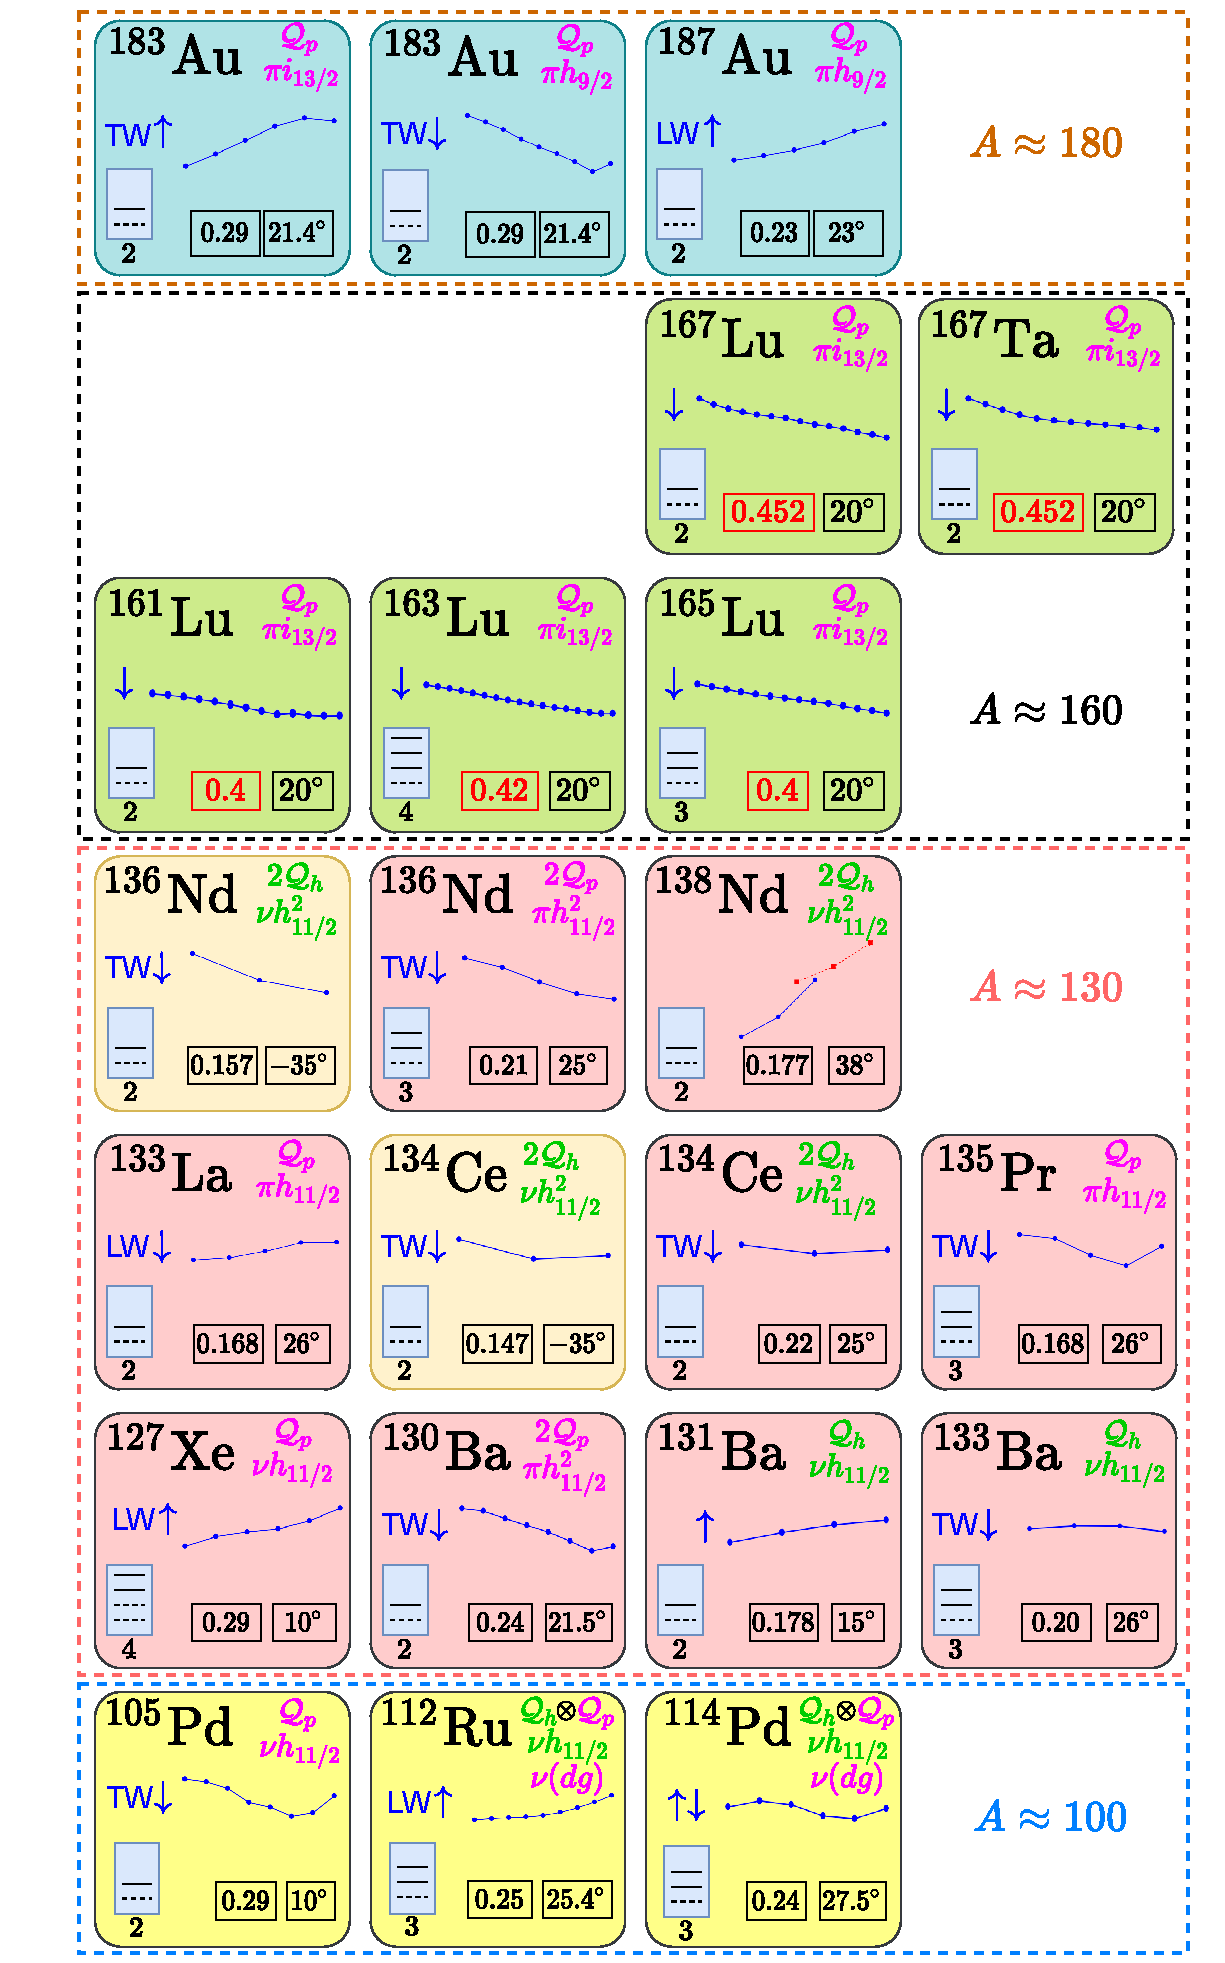
\includegraphics[scale=0.22]{Figs/wobblers-chart.pdf}
      \end{figure}
    \end{minipage}%
    \begin{minipage}{.5\textwidth}
      \par Wobbling nuclei (up to date)
      \par \textit{Poenaru, 2022, in progress}
    \end{minipage}
    \end{figure}
\end{frame}

%---------------------------------------------------------
\end{document}
%---------------------------------------------------------

% \begin{frame}
%   \frametitle{Highlighting text}
  
%   In this slide, some important text will be
%   \alert{highlighted} because it's important.
%   Please, don't abuse it.
  
%   \begin{block}{Remark}
%     Sample text
%   \end{block}
  
%   \begin{alertblock}{Important theorem}
%     Sample text in red box
%   \end{alertblock}
  
%   \begin{examples}
%     Sample text in green box. The title of the block is ``Examples".
%   \end{examples}
% \end{frame}